\documentclass[
    11pt, % Set the default font size, options include: 8pt, 9pt, 10pt, 11pt, 12pt, 14pt, 17pt, 20pt
    aspectratio=169, % Set aspect ratio to 16:9 widescreen
]{beamer}

\graphicspath{{Images/}{./}} % Specifies where to look for included images (trailing slash required)
\usepackage{booktabs} % Allows the use of \toprule, \midrule and \bottomrule for better rules in tables
\usepackage{xcolor}

%\usepackage{appendixnumberbeamer} %If you want a separate slide counter for your appendix

%%% Customize Theme %%%%%%%%%%%%%%%%%%%%%%
\usetheme{Madrid} % You can use other themes too, but this changes many things. I've found Madrid to be the best for this color scheme

\definecolor{myRed}{RGB}{120,4,4}
\definecolor{myOrange}{RGB}{227, 125, 0}

% Structure and Palette Colors
\setbeamercolor*{structure}{bg=myRed!20,fg=myRed}

\setbeamercolor*{palette primary}{fg=white,bg=myRed}
\setbeamercolor*{palette secondary}{fg=white,bg=myRed!85}
\setbeamercolor*{palette tertiary}{fg=white,bg=myRed!70}

% Slide Title & Header Bar
\setbeamercolor{frametitle}{bg=myRed,fg=white}

% Title Slide Header Box
\setbeamercolor{title}{bg=myRed,fg=white}
\setbeamercolor{subtitle}{fg=white}
\setbeamercolor{author}{fg=black}
\setbeamercolor{institute}{fg=black}
\setbeamercolor{date}{fg=black}
\setbeamertemplate{title page}[default][colsep=-4bp,rounded=true,shadow=true]

% Navigation Miniframes & Footer Bar
\setbeamercolor{section in head/foot}{fg=myOrange, bg=white}
\setbeamercolor{author in head/foot}{bg=myRed,fg=white}
\setbeamercolor{title in head/foot}{bg=myRed,fg=white}
\setbeamercolor{date in head/foot}{bg=myRed,fg=white}

% Specific Colors
\setbeamercolor{item projected}{bg=myOrange,fg=white}
\setbeamertemplate{enumerate items}[circle]
\setbeamercolor{itemize item}{fg=myOrange}
\setbeamercolor{itemize subitem}{fg=myOrange}
\setbeamercolor{button}{bg=myOrange}

% Table of Contents Styling
\setbeamercolor{section in toc}{fg=black}
\setbeamercolor{subsection in toc}{fg=black}
\setbeamercolor{section in toc projected}{bg=myOrange,fg=white}
\setbeamertemplate{sections/subsections in toc}[sections numbered]

% Block Colors
\setbeamercolor{block title}{bg=myOrange, fg=white}
\setbeamercolor{block body}{bg=myOrange!20}

%---------------------------------------------------------
%	SELECT FONT THEME & FONTS
%---------------------------------------------------------
\usefonttheme{default} % Typeset using the default sans serif font
\usepackage{palatino} % Use the Palatino font for serif text
%\usepackage[default]{opensans} % Open Sans is commented out to prevent compilation error if not installed on server
\useinnertheme{circles}
\useoutertheme{miniframes}

%---------------------------------------------------------
%	PRESENTATION INFORMATION
%---------------------------------------------------------

\title[Middle Footer]{Virginia Tech Presentation Template}
\subtitle{Subtitle}
\author[Left Footer]{Author: Jonathan Gendron}

\institute[]{Department of Economics \\ \smallskip \textit{email@vt.edu}}
\date[Fall 20XX]{Fall 20XX}

\logo{
\includegraphics[width=1.5cm]{Hokie2.png}}

%---------------------------------------------------------
\begin{document}

%---------------------------------------------------------
%	TITLE SLIDE
%---------------------------------------------------------
\begin{frame}
	\titlepage % Output the title slide
\end{frame}

%---------------------------------------------------------
%	TABLE OF CONTENTS SLIDE
%---------------------------------------------------------
\begin{frame}
	\frametitle{Table of Contents}
	
	\tableofcontents % Output the table of contents
\end{frame}

%---------------------------------------------------------
%	PRESENTATION BODY SLIDES
%---------------------------------------------------------
\section{Motivation} % Sections are added in order to organize your presentation into discrete blocks, all sections and subsections are automatically output to the table of contents as an overview of the talk but NOT output in the presentation as separate slides

%------------------------------------------------
\begin{frame}
	\frametitle{Title}
            \emph{To use this template, you can copy and just edit/add slides!}\newline

            This is because all the color customization occurs in the "Customize Themes" section in lines 12-51 of the code\newline

            The remainder of these slides serve an example to show all the features you can use: bullets, buttons, sections, etc.
\end{frame}

%------------------------------------------------
\begin{frame}
	\frametitle{Another Title}
	\framesubtitle{and a subtitle!}
	
	Look at the code of this slide to see how columns made this formatting look nice.

	\begin{columns}[t] % The "c" option specifies centered vertical alignment while the "t" option is used for top vertical alignment
		\begin{column}{0.5\textwidth} % Right column width
                \begin{figure}[h!]
                    \centering
                    %\caption{Hawkins et al, 2015}
                    
\includegraphics[angle=0, width=3cm]{Hokie2.png}
                    %\label{Figure 1}
                \end{figure}
		\end{column}
  		\begin{column}{0.5\textwidth} % Left column width
                \begin{figure}[h!]
                    \centering
                    %\caption{Hawkins et al, 2015}
                    
\includegraphics[angle=0, width=3cm]{Hokie2.png}
                    %\label{Figure 1}
                \end{figure}
		\end{column}		
	\end{columns}
\end{frame}

%------------------------------------------------
\begin{frame}
	\frametitle{Yet another title}
            You can use bullets too:\newline
            \begin{itemize}
                \item Like this one\newline
                \item \& this one
            \end{itemize}
\end{frame}

%------------------------------------------------
\begin{frame}
\label{Test} %For the link button for the Appendix slide
	\frametitle{A title}

        \begin{itemize}
            \item You can also nest sub-bullets
            \begin{itemize}
                \item Constant
                \item Cubic
                \item Continuous (with slope changes)
                \item Exponential \newline
            \end{itemize}
        \end{itemize}

        \textbf{Below is a button that links to a slide in the appendix}
        
        \begin{center}
            \hyperlink{Figure}{\beamergotobutton{Go to graphs}}    
        \end{center}
\end{frame}

%------------------------------------------------
\section{Theory}

%------------------------------------------------
\begin{frame}
\label{Test Stat}
	\frametitle{The Test Statistic}
		
        Here is a made up equation:
        $$ \hat{A} = \bar{m}-\hat{m}_S$$ \newline

        Notice how these buttons are centered and evenly spread out:\newline

        \begin{columns}[t] % The "c" option specifies centered vertical alignment while the "t" option is used for top vertical alignment
		\begin{column}{0.25\textwidth} % Right column width
                \hyperlink{Terms}{\beamergotobutton{Go to Terms}}
		\end{column}
  		\begin{column}{0.25\textwidth} % Left column width
                \hyperlink{Definitions}{\beamergotobutton{Go to Definitions}}
		\end{column}
            \begin{column}{0.25\textwidth} % Left column width
                \hyperlink{Theorems}{\beamergotobutton{Go to Theorems}}
		\end{column}
	\end{columns}
        
\end{frame}

%------------------------------------------------
\begin{frame}
	\frametitle{No way, another title!}
            \begin{enumerate}
                \item Instead of bullets, you can index by number too\newline
                \item like this
            \end{enumerate}
\end{frame}

%------------------------------------------------
\section{Testing}

%------------------------------------------------
\begin{frame}
	\frametitle{Second to last title}
    	\begin{block}{Block Title}
    		Block 1
    	\end{block}
    	
    	\begin{exampleblock}{Example Block Title}
    		Block 2
    	\end{exampleblock}
    	
    	\begin{alertblock}{Alert Block Title}
    		Block 3
    	\end{alertblock}
    	
    	\begin{block}{} % Block without title
    		Block without a title
    	\end{block}
\end{frame}

%------------------------------------------------
\section{Conclusion}
%------------------------------------------------
\begin{frame}
	\frametitle{Last title}
		
	Last bit of text

\end{frame}

%---------------------------------------------------------
%	CLOSING SLIDE
%---------------------------------------------------------

% To remove miniframe from top
\appendix
\setbeamertemplate{headline}{}
\addtobeamertemplate{frametitle}{\vspace*{-\headheight}}{}

\begin{frame}[noframenumbering] %So the end and appendix slides don't contribute to the page count
%[plain] % The optional argument 'plain' hides the headline and footline
	%\frametitle{Questions?}

	\begin{center}
            {\LARGE Questions?}
	\end{center}
 
\end{frame}
%---------------------------------------------------------

%------------------------------------------------
\begin{frame}[noframenumbering]
\label{Figure}
	\frametitle{Appendix - A figure}
        \hyperlink{Test}{\beamerreturnbutton{Return to presentation}}
        
        \begin{figure}[h!]
            \centering
            %\caption{}
            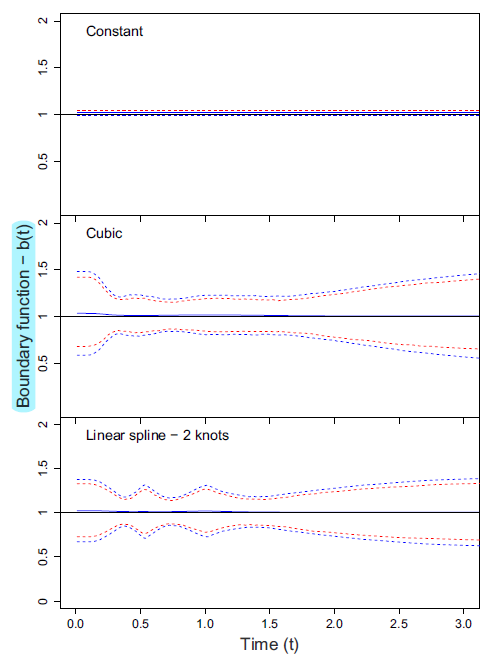
\includegraphics[angle=0, width=5cm]{Newey et al Graph.png}
            %\label{fig}
        \end{figure}
\end{frame}

%------------------------------------------------
\begin{frame}[noframenumbering]
\label{Terms}
	\frametitle{Appendix - Terms}

        \begin{columns}[t] % The "c" option specifies centered vertical alignment while the "t" option is used for top vertical alignment
		\begin{column}{0.5\textwidth} % Right column width
                Some Estimators:
                \begin{itemize}
                    \item Drift: $\hat{\delta}$
                    \item Boundary: $\hat{b}(t)$
                \end{itemize}
		\end{column}
  		\begin{column}{0.5\textwidth} % Left column width
                Some Variables:
                \begin{itemize}
                    \item $\hat{V}$
                    \item $\hat{m}_S$
                    \item $\bar{m}$
                    \item $m_J(\tau)$\newline\newline
                \end{itemize}
		\end{column}
	\end{columns}
        \hyperlink{Test Stat}{\beamerreturnbutton{Return to presentation}}        
\end{frame}

%------------------------------------------------
\begin{frame}[noframenumbering]
\label{Definitions}
	\frametitle{Appendix - Definitions}
         \begin{enumerate}
             \item A definition \newline
         \end{enumerate}
         
        \hyperlink{Test Stat}{\beamerreturnbutton{Return to presentation}}
\end{frame}

%------------------------------------------------
\begin{frame}[noframenumbering]
\label{Theorems}
	\frametitle{Appendix - Theorems}
         \begin{enumerate}
             \item A theorem\newline
         \end{enumerate}
         
        \hyperlink{Test Stat}{\beamerreturnbutton{Return to presentation}}        
\end{frame}

\end{document} 
